\chapter{Automated Segmentation of Kidneys using Machine Learning}
\label{chap:ML}

\begin{abstract}
	This work was presented as an aural presentation at the \ac{ISMRM} 28th Annual Meeting (2020) \cite{daniel_automated_2020}.\\
	
	\lipsum[1]
\end{abstract}
\newpage

\section{Introduction}

Segmentation of the kidneys in \ac{MRI} images is a vital, yet time consuming, aspect of many renal studies \cite{cohen_mri_2009, van_den_dool_functional_2005, cox_multiparametric_2017}. \ac{TKV} is used as a biomarker for a variety of renal pathologies; autosomal dominant polycystic disease is characterised by an increase in \ac{TKV} \cite{chapman_kidney_2012, tangri_total_2017}, while a decrease in \ac{TKV} is associated with a decrease in real function \cite{gong_relationship_2012}. In addition to \ac{TKV} measurements, renal segmentation is an important first step for many other processing pipelines, be that to increase accuracy of automated cortical-medullary segmentations or reduce computation times by only carrying out calculations for a relevant \ac{ROI}. The gold standard of segmentation is manual \ac{ROI} definition by an experienced and skilled professional, this manual process is highly time consuming and difficult due to similar signal intensities between the kidneys and other organs, anatomical differences between subjects and imaging artefacts. These factors mean that developing a fully automated method of renal segmentation is highly desirable. Such methods have been proposed with varied successes \cite{zollner_assessment_2012, seuss_development_2017} however the techniques used differ between diseases. The fact that each technique is highly optimised for a specific dataset means that it needs to be re-written to be applied to different a pathology, another time consuming and highly skilled process.\\

Machine learning allows for a single method to be written and then trained on different datasets. This means that as more data becomes available the algorithm can become more accurate and generalised, without a need to rewrite the methods, thus making it a better choice for long term development. Such methods have already been applied to segmentation in other areas of medical imaging, especially successful have been U-Nets. An example of a \ac{FCN}, these algorithms convolve the image with a series of filters to extract features from the input data and thus generate a voxel by voxel classification. The weights of each pixel in these convolution kernels is honed through an optimisation process where the filters are applied to the training data and their performance is evaluated against the manually segmented data using a loss function such as mean square error or dice overlap score. Changes to each filter are then back propagated through the network and the process starts again. After many iterations, the filters become tuned to detecting the feature labelled in the manually segmented data.\\ 

To avoid the network becoming too specific and, for example, just learning to detect the specific kidneys in the data the network has been trained on rather than all kidneys, the data is divided into three categories, training, testing and validation. The training data is used for adjusting the filter weights over a short time scale, usually after a few tens of images. Once all the training data has been processed by the network and filter weights adjusted, all the test data is run through the network without any further weight adjustments and the performance evaluated using the loss function, this train, test cycle is known as an epoch. If the network has become too specialised and finely adjusted to the training data then it will not perform well on the test data. To stop this over specialisation, or over-fitting, the weights used at the start of each epoch are those that delivered the best performance on the test data. The validation data is never used to influence the filter weights and is used to validate the performance of the network on unseen data.\\

Similar methods have been applied to segment other areas of anatomy \cite{wachinger_deepnat_2018, lu_automatic_2017}, however this has not been successfully applied to segment the kidneys. Here we propose a \ac{FCN} to segment the kidneys from a standardised \ac{MRI} protocol.

\newpage
\section{Methods}

\subsection{Data Acquisition}
\label{sec:ml_methods_acquisition}
All data is acquired on a 3T Philips Ingenia system using a $T_2$-weighted \ac{HASTE} sequence (\ac{TE} = 60, \ac{TR} = 1800 or 1300 ms, \ac{FOV} = 350 $\times$ 350 mm$^2$, voxel size = 1.46 $\times$ 1.46 $\times$ 5 mm$^3$ with enough slices to cover the entire kidney, usually 12-14, \ac{SENSE} = 2.5), the sequence is carried out in a single breath hold. Parameters have been optimised to deliver the maximum contrast between the kidneys and surrounding tissue. Training and test data is a single volume per subject; validation datasets are composed of five volumes acquired on the same subject in the same scanning session with the subject being removed from the scanner, asked to move, then positioned back in the scanner between each acquisition. The scanner operator attempted to vary the acquisition geometry between repeats while still acquiring the full kidney volume. These validation datasets allow the consistency of the networks ability to measure \ac{TKV} to be assessed. Manual binary masks are generated for every volume to allow the network to train and its accuracy to be investigated. A summary of the data collected can be seen in Table \ref{tab:ml_data}, to make the algorithm as generalisable as possible, healthy volunteers and patients with \ac{CKD} are scanned.\\

\begin{table}[H]
	\centering
	\begin{tabular}{|l|l|l|}
		\hline
		\textbf{Dataset}           & \textbf{Number of Subjects} & \textbf{Number of Volumes} \\ \hline
		Healthy kidneys            & 26                            & 26                         \\ \hline
		\ac{CKD} kidneys           & 23                            & 23                         \\ \hline
		Validation healthy kidneys & 5                             & 25                         \\ \hline
		Validation \ac{CKD} kidneys& 3                             & 15                         \\ \hline
	\end{tabular}
	\caption{Number of subjects and volumes in each dataset type.}
	\label{tab:ml_data}
\end{table}

The accuracy of the network will increase as it is trained on a greater volume of data. As such, this protocol is still being run on as many subjects as possible to further increase the accuracy of the algorithm.

\subsection{Data Pre-Processing}
All training and test data is loaded and the order of the volumes randomised i.e. healthy volunteers and patients are mixed. Each slice is resampled to a matrix size of 256 $\times$ 256 and voxel intensities scaled between 0 and 1 where black is set to the mean voxel value minus 0.5 times the standard deviation of that slice and white is set to the mean voxel value plus 4 times the standard deviation of the slice; values outside this range are clipped to 0 or 1. This windowing leads to a clear contrast between kidneys and surrounding tissue while negating the effects of bulk signal changes between subjects.\\

This resampling and windowing is also applied to the validation data before it is processed by the network. Once a prediction of the renal mask has been generated by the algorithm, the mask is resampled back to the original image volume dimensions.\\

The ratio of training data to test data is eighty to twenty. No data augmentation is performed in this architecture.\\

\subsection{Network Architecture}

A summary of the network architecture is shown in Figure \ref{fig:ml_network}. Each volume is split into two-dimensional slices before being processed by the network. Convolution and deconvolution layers use a 3 $\times$ 3 kernel. Activation layers use a \ac{ReLU}. Max pooling with a stride 2 is used on the encoding half of the network.

\begin{figure}[h]
	\centering
	\includegraphics[width=1\textwidth]{ML/Model/Model.eps}
	\caption{The architecture of the network used.}
	\label{fig:ml_network}	
\end{figure}

The network uses a dice score, defined by Equation \eqref{eq:dice}, as its loss function; this function is ideal for renal segmentation as it doesn't weight true negatives which represent the majority of voxels input to the network. Training is carried out over 150 epochs using stochastic gradient decent with a learning rate of 0.01 to optimise the networks approximately thirty million trainable parameters.

\begin{equation}
D\left(A, B\right) = \frac{2\left| A \cap B \right|}{\left|A\right|+\left|B\right|}
\label{eq:dice}
\end{equation}
The network is implemented using Keras \cite{chollet_keras_2015} with a TensorFlow \cite{abadi_tensorflow_2015, martin_abad_tensorflow_2019} back-end and is trained on an NVIDIA Titan Xp \ac{GPU}. Training takes approximately forty minutes for the 150 epochs and predicting a renal mask from a thirteen slice volume takes approximately 9 seconds when executed on a computer with no \ac{GPU} (as it would be in most end user cases).

\newpage
\section{Results and Discussion}

Initial data was collected with a \ac{TR} of 1800 ms leading to a breath hold of approximately 23 seconds. Some subjects struggled to hold their breath for this long on expiration, therefore the effects of reducing the \ac{TR} of the sequence were investigated. As can be seen in Figure \ref{fig:ml_tr}, there is no degradation in image quality from the image with \ac{TR} or 1800 ms to that with at \ac{TR} of 1300 ms, the differences between these images are mainly due to the small movements between volumes, as can be seen in the difference data where the largest differences are seen around the periphery of the kidneys and in the gut. Moving forward, the \ac{TR} was reduced to 1300 ms leading to a sequence with a breath hold of approximately 17 seconds.

\begin{figure}[H]
	\centering
	\includegraphics[width=1\textwidth]{ML/TR/TR_Master_V0_1.eps}
	\caption{The effects of changing the \ac{TR} of the sequence.}
	\label{fig:ml_tr}	
\end{figure}

To verify that the trained network is behaving as expected saliency maps were produced, Figure \ref{fig:ml_salency}, this is especially important given the black box nature of machine learning methods. This map shows the areas the network is using most in its classification \cite{mahapatra_visual_2016}. It verifies that the networks is using the outside areas of the kidney to make its prediction with areas of a similar intensity receiving some attention to distinguish them from the kidney. While this is precisely what is expected of the algorithm, it is important to check this as it is possible for such a method to have learnt a slightly different mechanism for the segmentation, one that is more prone to errors if new data is presented to it.

\begin{figure}[H]
	\centering
	\includegraphics[width=.4\textwidth]{ML/Salency/MSE_Salency.png}
	\caption{An example saliency map of the areas the network uses most when segmenting the kidney.}
	\label{fig:ml_salency}	
\end{figure}

To assess the accuracy of the network, each of the five volumes per validation subject was segmented by the trained network, in theory the \ac{TKV} predicted for each volume should have been the same. Figure \ref{fig:ml_validation} shows the predicted \ac{TKV} against the manually segmented ``true" \ac{TKV} with each subject plot in a different colour. While there is a spread in the predicted values, there is also a reasonable variation in manual \ac{TKV}. For three out of the seven repeatability subjects, the predicted \ac{TKV} has a smaller standard deviation than the manually segmented data, this indicates that the algorithm may actually be more consistent than the humans. To identify if a systematic error is present, a Bland-Altman plot was generated (Figure \ref{fig:ml_ba_validation}). From this figure it is possible to see that the algorithm is slightly over estimating the \ac{TKV} by 0.69\% (1.6 mm$^3$) but there is no correlation between difference in \ac{TKV} and true \ac{TKV} over all subjects. There is a more subtle trend between each repeat on the same subject though, the volumes with a smaller true \ac{TKV} are consistently over estimated more than those volumes with a larger true \ac{TKV}. This again points to an issue with the manual segmentation rather than the algorithm.

\begin{figure}[H]
	\centering
	\begin{subfigure}[c]{0.47\textwidth}
		\centering
		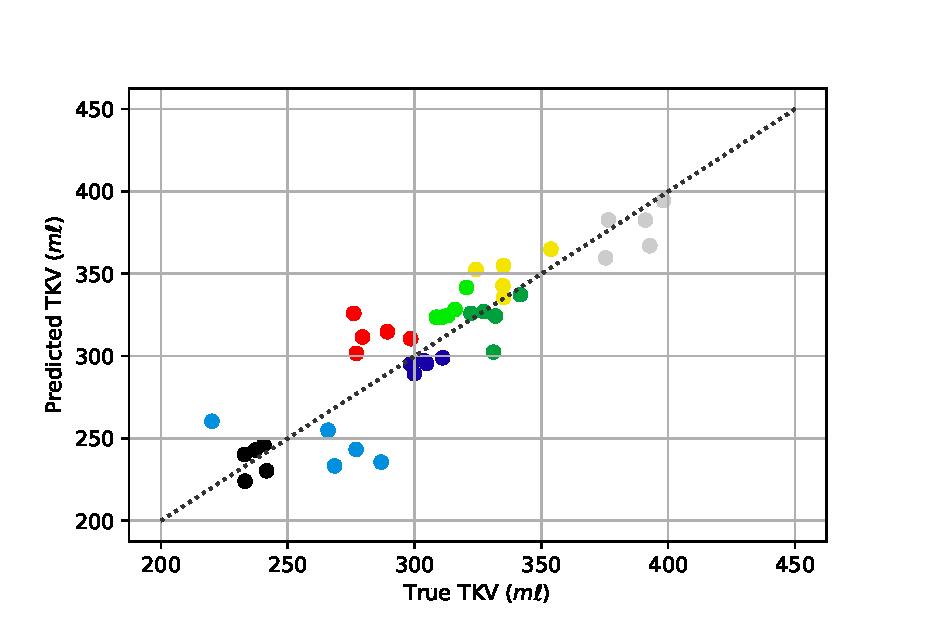
\includegraphics[width=1\textwidth]{ML/BA_plots/190802_training_data_shuffle_input_and_slices_max_dice_09013_validation_tkv.eps}
		\caption{}
		\label{fig:ml_validation}
	\end{subfigure}
	\hfill
	\begin{subfigure}[c]{0.47\textwidth}
		\centering
		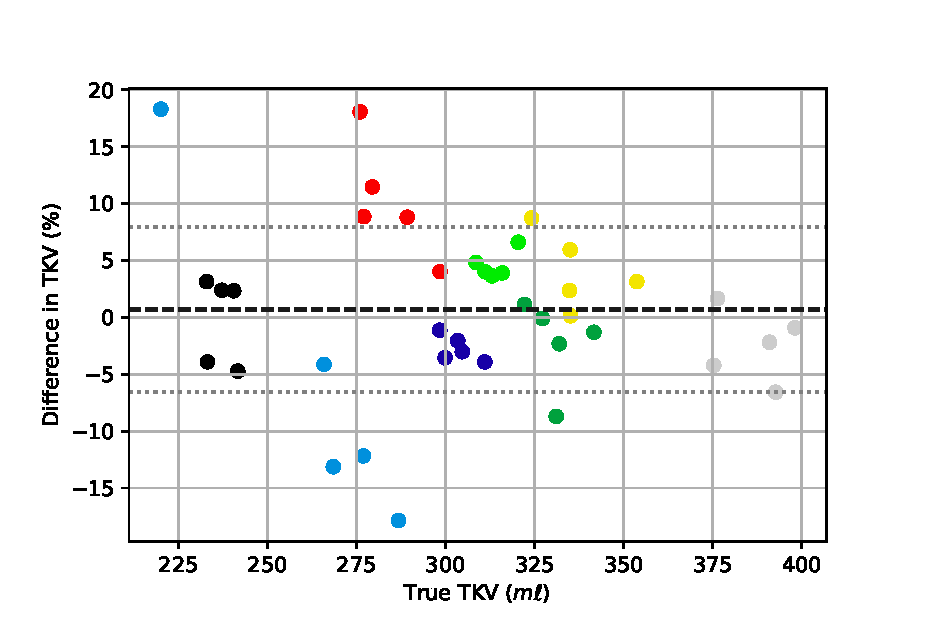
\includegraphics[width=1\textwidth]{ML/BA_plots/190802_training_data_shuffle_input_and_slices_max_dice_09013_validation_ba.eps}
		\caption{}
		\label{fig:ml_ba_validation}
	\end{subfigure}
	\caption{(\subref{fig:ml_validation}) The predicted \ac{TKV} plot against the manually segmented ``true'' \ac{TKV}. Each subject is plot in a different colour. (\subref{fig:ml_ba_validation}) A Bland-Altman plot to identify and systematic error in the networks performance. Each subject is plot in a different colour.}
	\label{fig:ml_validation_tkv}
\end{figure}

While assessing the ability of the algorithm to predict \ac{TKV} is important, it is also necessary to access the raw segmentation as, for example, the algorithm may be over-estimating the size of central slices but under-estimating the size of edge slices. This type of inaccuracy could be masked in the \ac{TKV} however will be visible in the dice scores. These are shown in Figure \ref{fig:ml_validation_dice}.

\begin{figure}[H]
	\centering
	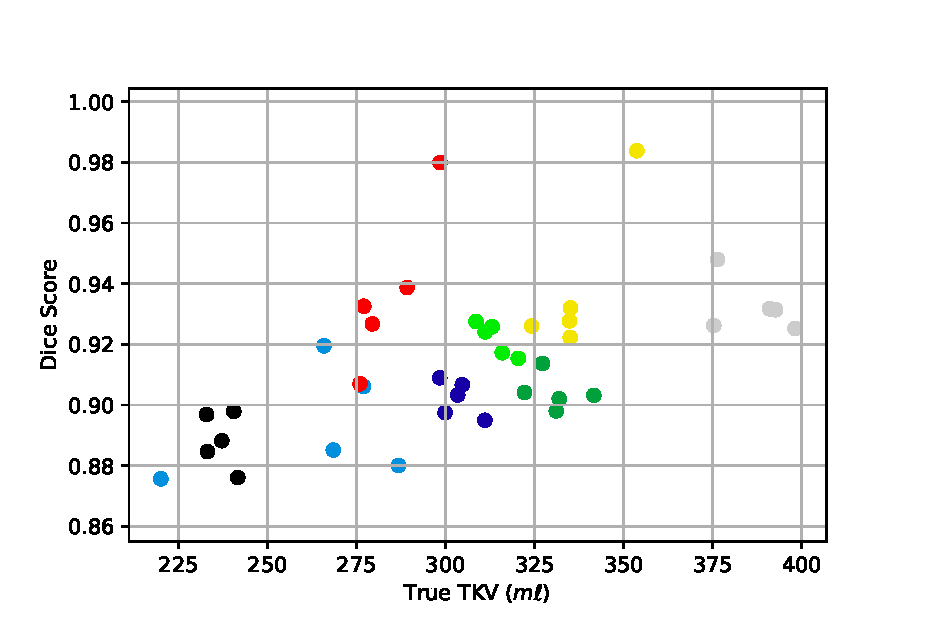
\includegraphics[width=.47\textwidth]{ML/BA_plots/190802_training_data_shuffle_input_and_slices_max_dice_09013_validation_dice.eps}
	\caption{The dice scores for all volumes in the validation data. Each subject is plot in a different colour.}
	\label{fig:ml_validation_dice}
\end{figure}

The mean dice score over all forty volumes is 0.91$\pm$0.02. Here we see a slight trend towards more accurate predictions for larger kidneys. The reason for this becomes clear when we look at the \ac{ROI} the algorithm is outputting, Figure \ref{fig:ml_roi}.

\begin{figure}[H]
	\centering
	\begin{subfigure}[c]{0.47\textwidth}
		\centering
		\includegraphics[width=1\textwidth]{ML/ROI/Kidney_vols2_repro3_T2W_TSE_Cor_BH_60_2_1_sl_01.png}
		\caption{}
		\label{fig:ml_roi_outside}
	\end{subfigure}
	\hfill
	\begin{subfigure}[c]{0.47\textwidth}
		\centering
		\includegraphics[width=1\textwidth]{ML/ROI/Kidney_vols2_repro3_T2W_TSE_Cor_BH_60_2_1_sl_08.png}
		\caption{}
		\label{fig:ml_roi_inside}
	\end{subfigure}
	\caption{(\subref{fig:ml_roi_outside}) A slice from the posterior of the volume. (\subref{fig:ml_roi_inside}) A slice from the centre of the kidneys.}
	\label{fig:ml_roi}
\end{figure}

In Figure \ref{fig:ml_roi_outside} the algorithm is assigning false positives on the right hand side of the image in the area a kidney would be expected further into the body. The amount of false positives decrease as the slices move in an anterior direction as kidney comes into the slice, \ref{fig:ml_roi_inside}. The algorithm works on each slice individually as a two-dimensional image rather than as a three-dimensional volume. This means that, as the majority of slices in the training data have two kidneys in them, the algorithm is more likely to generate false positives if there is no kidney in the slice. For smaller kidneys, there are more slices with no kidney in them and therefore the overall dice score is lower, hence the trend observed in Figure \ref{fig:ml_validation_dice}.\\

There are multiple methods of reducing this tendency in the algorithm. The false positives tend to be spatially independent through slices, this means that it would be relatively simple to remove them in post-processing by reconstructing the two-dimensional slices back into a three-dimensional volume and removing masked areas with a small volume or areas that are very thin in the anterior-posterior direction. Another method would be to modify the architecture to a \ac{RNN} with \ac{LSTM}. This would also keep the large advantage of working with two-dimensional images, that the algorithm generalises to $n$ slices, but means that the algorithm also has some memory of what is in the surrounding slices \cite{chen_combining_2016, stollenga_parallel_2015}. Finally the algorithm could be re-written as a three-dimensional \ac{FCN}, this would give the greatest degree of accuracy between slices however comes at the expense of simple generalisation with regards to number of slices or the slice thickness and would require much more data collection as amount of training/test data would be reduced by a factor of approximately thirteen.\\

To establish how the network is performing with the relatively small amount of training data, predictions were made on the training and testing data and the dice score plot, Figure \ref{fig:ml_training_dice}.

\begin{figure}[H]
	\centering
	\includegraphics[width=.5\textwidth]{ML/BA_plots/190802_training_data_shuffle_input_and_slices_max_dice_09013_training_dice.eps}
	\caption{The dice score of predictions made on the training data.}
	\label{fig:ml_training_dice}
\end{figure}

The algorithm is performing better on most of the training data than it did on the validation data although with 80\% of the volumes segmented more accurately than the validation data. This indicates that a certain degree of over fitting is occurring as the 20\% of volumes that are not segmented as well are most likely the testing data. Earlier in the development of this network it was established that augmentation did not improve the performance of the trained network however this should be explored again in light of this result as some basic augmentation would lead to a smaller disparity between the training data and test data and thus allow for better performance when segmenting the validation data.\\

An indication that some degree of data augmentation would be beneficial is also seen when investigating if there is any difference in performance of the network between healthy and \ac{CKD} kidneys. The manually segmented mean \ac{TKV} of the healthy subjects is 330$\pm$35 m$\ell$ and for subjects with \ac{CKD} is 268$\pm$32 m$\ell$ therefore it would be expected that the algorithm would perform better on the healthy subjects given their larger kidney volume. This is not the case though, the mean dice score of the validation images for healthy kidneys is 0.89$\pm$0.02 and for kidneys with \ac{CKD} this increases to 0.93$\pm$0.02. As there are more healthy subjects in the training data (26 versus 23) it would be expected that the network would perform better for these subjects however the greater degree of variability in geometry and size of the \ac{CKD} kidneys means they essentially have some degree of augmentation built into them. If this were replicated via data augmentation in the whole training dataset then an increase in accuracy across the board may be observed.\\

\newpage
\section{Conclusions and Future Work}

This method has been shown to produce promising results delivering an mean dice score of 0.91$\pm$0.02 over eight unseen scans with a mixture of healthy and \ac{CKD} subjects resulting in a mean \ac{TKV} difference of 0.69\% when compared to the manually segmented \ac{TKV}. This is especially promising as the algorithm will improve in accuracy as more training data is collected, something which the renal group at \ac{SPMIC} are actively pursuing by adding this scan to almost every subject that goes in the scanner. Efforts have been made to avoid the quintessential machine learning mistakes such as imbalanced training data making the algorithm too specific and un-generalisable and the network only working for healthy subjects. We have also peaked inside the black box of the algorithm to check that it is behaving in a sensible and expected manner.\\

There is still work to be done on this segmentation method, as explained above, there are signs that data augmentation may improve both the accuracy and generalisability of the algorithm, this should be implemented and evaluated. By implementing data augmentation, the false positives observed on fringe slices may decrease however, if this is not the case then there are multiple solutions to reduce the prevalence of these errors such as basic binary filtering or modifying the networks architecture. There seems to be a reasonable degree of variability in the manually segmented data, to investigate this, the manual masking process should be repeated by a second observer at assess if this variability in the data is due to acquisition or human interpretation.\\

Another common segmentation task in renal imaging is to generate \ac{ROI} for the renal cortex and medulla. There are some automated methods of achieving this once an overall renal mask has been produced \cite{cox_multiparametric_2017}, however there has been no work on the application of machine learning to this task. During the acquisition of the $T_2$ weighted data in Section \ref{sec:ml_methods_acquisition}, a sequence designed to optimise the contrast between cortex and medulla was also collected on each subject, an example of which is shown in Figure \ref{fig:ml_t1}. Using this data it may be possible to develop the algorithm further so it can segment each tissue type within the kidneys.

\begin{figure}[H]
	\centering
	\includegraphics[width=.4\textwidth]{ML/T1/T1W.png}
	\caption{An example of the data collected to enable segmentation of the renal cortex and medulla.}
	\label{fig:ml_t1}
\end{figure}

Ultimately the goal of this work is to produce an easy to use segmentation tool that can be utilised by clinicians and scientists alike. As such, time should be spent making the software easy to use with a simple front end/\ac{GUI}.

\section{Acknowledgements}

We gratefully acknowledge the support of NVIDIA Corporation with the donation of the Titan Xp GPU used for this research.\\

\newpage
\section{References}
\defbibheading{bibliography}[\refname]{}
\printbibliography